% com-cas
% by hk, rj, January 2012

\documentclass{llncs}

%create pdf images with epstopdf not ps2pdf

%todo:

\usepackage{epsfig}
%\usepackage{graphicx}
\usepackage{amssymb}
%\usepackage{amsmath}
%\usepackage{amsfonts}

\addtolength{\textheight}{1.5cm}

\newcommand{\code}[1]{\texttt{#1}}
\raggedbottom

\begin{document}

\title{Categories as classes and mixin composition}

\author{Heinz Kredel\inst{1} and Raphael Jolly\inst{2}} 
\institute{IT-Center, University of Mannheim, Germany,
\email{kredel@rz.uni-mannheim.de,}
\and Databeans, Paris, France,
\email{raphael.jolly@free.fr}}

\maketitle

\begin{abstract} 
  The modeling of algebraic structures in a strongly typed, generic,
  object oriented computer algebra software has been presented with
  the systems JAS and ScAS. These systems exemplify the design and
  implementation of strongly typed, generic and object oriented
  polynomial algorithm libraries in Java and Scala. The libraries have
  grown over the time by several algorithm versions for greatest
  common divisor, squarefree decomposition, factorization and
  Gr\"obner bases computation in separate packages. In this paper we
  discuss the problem of code organization and algebraic structure
  configuration and deployment.  In search of a possible solution we
  study the category concept in Magma and Sage and propose a novel
  code organization scheme using mixin composition. The resulting code
  is again strongly typed, generic and object oriented.
\end{abstract}

%\keywords{object oriented programming, generic type-safe library,
%mixin composition, categories}


\section{Introduction} %------------

The modeling of algebraic structures in a strongly typed, generic,
object oriented computer algebra software has been presented with the
systems JAS \cite{Kredel:2008} and ScAS \cite{Jolly:2010}. %Kredel:2000,
The design and implementation of these strongly typed, generic and
object oriented polynomial algorithm libraries in Java and Scala is
presented in \cite{JollyKredel:2010,JollyKredel:2011}.  The libraries
are enhanced for interactive usage with the help of the Jython and
JRuby scripting languages \cite{JollyKredel:2009}.  The libraries now
provide several algorithm versions for greatest common divisor,
squarefree decomposition, factorization and Gr\"obner bases
computation in separate packages \cite{Kredel:2011}.

In this paper we discuss the problem of code organization and
algebraic structure configuration and deployment. Elements of algebraic
structures are implemented by classes and instantiated as objects with
methods implementing the `inner' algorithms of the structure in the
programming language. The algorithm libraries, for example the
construction of Gr\"obner bases, are kept in separate source code trees
and packages. This code organization helps in the separation of the
various possibilities for algorithm implementation and helps in the
transparent selection of appropriate algorithms for a given problem.
However, it is not always clear where to draw the line between `inner'
structure algorithms and `external' library algorithms.

In search of a possible solution we study the category concept in
Magma \cite{BosmaCannonPlayoust:1997} and Sage \cite{Stein:2005} and
compare it to our approach. In the comparison we focus on the computer
science aspects and ignore the mathematical scope of the systems as
well as some questions related to the software architecture, like
run-time infrastructure with automatic memory management and scripting
languages for interactive use, we also do not elaborate on performance
aspects.
%
We propose a new concept to provide library code organization
using mixin composition. The new category concept combines algebraic
structures and configurations of optimally suitable algorithm
implementations based on properties of the incorporated basic
algebraic structures.  The resulting code is again strongly typed,
generic and object oriented.


\subsection{Related work} % -----------------------------------

As we provide a detailed comparison with Magma
\cite{BosmaCannonPlayoust:1997} and Sage \cite{Stein:2005} with
comments on {\em Axiom} \cite{JenksSutor:1992,Watt:2003} in section
\ref{sec:compare}, we will mention related work there.
%Further related work is mentioned in the paper as required.


\subsection{Outline} % -----------------------------------

The paper is organized as follows : Section \ref{sec:asto} introduces
our generic, strongly typed, object oriented computer algebra
software. A comparison with the computer algebra systems Magma and
Sage is then made in Section \ref{sec:compare}, where the concept of
categories as used in Magma, is summarized. Lastly, Section
\ref{sec:mixin} shows how in our software, algorithm implementations
can be packaged and re-combined using traits in a category-like
fashion.

\section{Generic, strongly typed, object oriented computer algebra software} % -----------
\label{sec:asto}

In this section we give an introduction into the object oriented
strongly typed generic software libraries. For more details see our
earlier articles and implementations
\cite{Kredel:2008,Jolly:2010,JollyKredel:2010,JollyKredel:2011,JollyKredel:2009,Kredel:2011}. %Kredel:2000,
%
First we discuss the design of interfaces to capture the functionality
of ring elements and so called ring factories, as examples for the
representation of algebraic structures. Then we summarize the design
and implementation of our main data structure, namely polynomials and
polynomial rings. Finally we give an overview on important parts of
our algorithm libraries, namely greatest common divisors, squarefree
decomposition and factorization of polynomials.


\subsection{Ring elements, ring factories and polynomial rings} %------------
\label{sec:ring}

The basic building blocks of the type system consists of the
interfaces \code{RingElem} and \code{RingFactory} and the classes
which implement them, see figure \ref{fig:bastype}. \code{RingElem}
defines the methods which we expect to be available on all ring
elements, for example \code{multiply()},
\code{isZERO()} or \code{isUnit()} with the obvious meanings. The
construction of ring elements is done by factories, modeled after the
{\em abstract factory} creational design pattern \cite{Gamma:1995}.
The factory \code{RingFactory} defines the construction methods for
elements, for example \code{get\-ONE()} to create the one element from
the ring, 
%\code{from\-Integer()} to embed the natural numbers into the ring, \code{subtract()},
%\code{random()} to create a random element 
\code{parse()} to create an element from a string representation or query methods such as
\code{is\-Asso\-ciative()}. % to query if the ring is associative. 

\begin{figure}[thb]
\centering
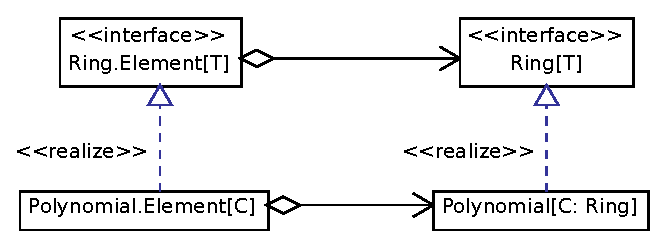
\epsfig{file=BasicTypes,clip=,width=0.55\linewidth}
%\\
\caption{Basic types}
\label{fig:bastype}
\end{figure}

%\subsection{Polynomials and polynomial rings} %------------

The polynomial class \code{Gen\-Polynomial} with type parameter
\code{C} for the coefficient type implements the \code{Ring\-Elem}
interface and specifies that coefficients must be of type
\code{Ring\-Elem}.  In addition to the methods mandated by the
interface, \code{Gen\-Polynomial} implements methods like
\code{leading\-Monomial()} or \code{degree()}.  Polynomials are to be
created with a polynomial factory \code{Gen\-Polynomial\-Ring}. In
addition to the ring factory methods it defines for example methods
to create random polynomials.  The constructor for
\code{Gen\-Polynomial\-Ring} takes parameters for a factory for the
coefficients, the number of variables, the names for the variables and
a term order object \code{Term\-Order}. The relation between the
factory of the coefficients and the polynomial ring factory is modeled
after the (constructor) dependency injection pattern and implements the
inversion of control principle.

Figure \ref{fig:bastype} shows dependency arrows from the factories to
the element interfaces as factories create the respective elements.
%The modeling of the constructors is not shown as it is not denotable
%with Java interfaces. 
The constructors of ring elements implement an opposite
dependency : each constructor takes a corresponding ring
factory as parameter.  It is only indirectly enforced since the
\code{RingElem} interface specifies a method \code{factory()} to
obtain the corresponding factory.
% So methods on ring elements have access to the corresponding
% factory for construction of new elements.

The factory methods are not static 
%(which is apparent from the modeling as an interface) 
since a ring factory might depend on other rings or specific
parameters. In case of a polynomial factory it depends on a factory
for the coefficients and at least the number of variables of the
polynomial ring. By this modeling the types of elements of algebraic
structures are not simply denoted in the program text but have to be
created as programming objects (by instantiating the respective
classes). Type denotations show up explicitly in Java program code and
are mostly inferred in Scala via type resolution. In Scala we have
experimented with elements as static inner classes of factories
and vice versa, which results in a slightly different naming, but is
otherwise equivalent.

For example a polynomial $w^2 - 2 \in \mathbb{Q}[w]$ can be
constructed by first constructing an object for the ring
$\mathbb{Q}[w]$ and then reading and constructing the polynomial $w^2
- 2$ with the factory method \code{parse()}.
{\small
\begin{verbatim}
  BigRational rf = new BigRational(1); // here element = factory
  GenPolynomialRing<BigRational> pf 
   = new GenPolynomialRing<BigRational>(rf,new String[]{ "w" });
  GenPolynomial<BigRational> a = pf.parse("w^2 - 2");
\end{verbatim}
}
%This example is continued in Subsection ?. %\ref{sec:anqf}.


\subsection{Algorithm libraries} %------------
\label{sec:algo}

We focus on algorithms for multivariate polynomials in (constructive)
unique factorization do\-mains.  Other algorithms, for example Gr\"ob\-ner
bases, comprehensive Gr\"obner bases, real and complex root isolation,
univariate power series and elementary integration of rational
functions are discussed elsewhere. %\cite{Kredel:2000,Kredel:2009,Kredel:2009a}.  
%For the mathematical background see some text books on the topic, like
%\cite{GeddesCzaporLabahn:1993}. %--++ zur Gathen, Kaltofen.
%
We give an overview of the respective interfaces and classes of the JAS
implementation. 

We start with an interface \code{Greatest\-Common\-Divisor}.  It
defines the method names for a ring with gcd algorithm.  First there
is the method \code{gcd()} itself, together with the method
\code{lcm()} to compute the least common multiple of two polynomials.
With the help of \code{gcd()} the algorithms for the content
\code{con\-tent()} and the primitive part \code{primitive\-Part()}
computation can be implemented.
%
The methods \code{coPrime()} compute lists of
co-prime polynomials from given lists of polynomials.

% The abstract super class for the implementations is called
% \code{Greatest\-Common\-Divisor\-Abstract}. It implements nearly all
% methods defined in the \code{Greatest\-Common\-Divisor} interface.
% The abstract methods are \code{base\-Gcd()} and
% \code{recursive\-Uni\-vari\-ate\-Gcd()}.  The method \code{gcd()}
% first checks for the recursion base, and eventually calls
% \code{base\-Gcd()}.  Otherwise it converts the input polynomials to
% recursive representation, as univariate polynomials with multivariate
% polynomial coefficients, and calls method
% \code{recursive\-Uni\-vari\-ate\-Gcd()}.  

The concrete implementations come in two flavors.  The first flavor
implements only the methods \code{base\-Gcd()} and
\code{recursive\-Univariate\-Gcd()}, using the setup provided by the
abstract super class.  There are implementations for various
polynomial remainder sequence (PRS) algorithms: simple, monic,
primitive and the sub-resultant algorithm (in the respective classes).
These implementations are generic for any (UFD) coefficient ring.  The
second flavor directly implements \code{gcd()} without providing
\code{base\-Gcd()} and \code{recursive\-Univariate\-Gcd()}.  The
algorithms compute gcds first modulo some suitable prime numbers and
then interpolate the result using Chinese remainder algorithms, or in
the Hensel case via powers of the prime number.  
%The later versions are
%only valid for integer or modular coefficient classes
%\code{Big\-Inte\-ger}, \code{Mod\-Integer} or \code{Mod\-Long}.

A similar design is used for squarefree decomposition where we have to
distinguish three major and two sub cases: coefficient fields of
characteristic zero, and coefficients not from a field. For
coefficient fields of characteristic non-zero we need two sub-cases
and classes for finite and infinite fields.

For polynomial factorization the design must reflect the fact that
factorization strongly depend on the respective coefficient ring.  At
least the factorization of a square-free univariate polynomial (an
abstract method) must be implemented for each coefficient ring.  For
multivariate polynomials Kronecker's algorithm is used to reduce this
case to a univariate problem and to reassemble multivariate factors
from univariate ones. For integer coefficients there is now also the
algorithm of Wang which uses a multivariate Hensel lifting algorithm.
The factorization algorithm is generic in the sense that it can factor
over arbitrary stacked coefficient field extensions, like mixed
transcendental and algebraic extensions, of some existing base field,
for which a factorization is available.

The selection of a suitable algorithm implementation for any given
coefficient field and polynomial ring is handled by the
algorithm factories \code{GCD\-Factory}, \code{Squarefree\-Factory} and
two \code{Factor\-Factory} classes. Each factory has at least methods
\code{get\-Implemen\-tation(cofac)} for different coefficient ring
factories \code{cofac}.

{\bf Problem:} The algebraic structures and elements of them together
with the algorithm libraries provide a precise way to use a suitable
combination for a given situation. It is, however, elaborate and one
would like to combine or package together certain configurations to be
able to deploy and use them as a single object or thing. In section
\ref{sec:mixin} we will sketch a solution to this problem.


\section{Comparison with Magma and Sage} % --------------------------------
\label{sec:compare}

In this section we discuss and compare the Magma, based on
\cite{BosmaCannonMatthews:1994,BosmaCannonPlayoust:1997}, and the
Sage, see \cite{Stein:2005,SageWiki:2009}, computer algebra systems to
our JAS and ScAS approach. We focus on the computer science aspects
and deliberately ignore performance aspects and mathematical scope of
the systems.
%
As Sage aims to provide an open source alternative to Magma
\cite{SageWiki:2009}, we first give a summary of the computer science
of mathematical concepts of Magma and then look into the Sage
implementation.


\subsection{Magma} % --------------------------------

In the ``Theoretical Foundations'' of \cite{BosmaCannonPlayoust:1997}
the concepts from {\em Universal Algebra} are named as basis for the
interaction and programming language of Magma. They use order
respectively multi sorted $\Sigma$-algebras for types and provide
homomorphic images of $\Sigma$-algebras, sub-$\Sigma$-algebras,
quotient $\Sigma$-algebras and direct products of $\Sigma$-algebras.
%
However, $\Sigma$-algebras are restricted to $\Sigma$-varieties
($\Sigma$-algebras closed under sub-structure, homomorphic image and
direct product construction).
% (hence also closed under quotient structures)
Although $\Sigma$-varieties have nice mathematical properties - they
can be defined by an equational theory
%\footnote{by a theorem of Birkhoff} 
- many important algebraic structures are not
varieties. For example the class of fields (of fixed characteristic)
are not a variety because they are not closed under direct products.
So we do not see a rationale for that design decision.

$\Sigma$-algebras are then organized according to concepts from {\em
  category theory} with objects (carrier sets), morphisms, composition
of morphisms and functors between categories. Magma focuses on the
existence of free algebras (generated by some set $X$) to construct
such structures in the interaction language. The existence of
generators then allows the construction of quotients of free algebras
and the representation of homomorphisms via images of generators.

The Magma {\em computational model} starts from $\Sigma$-varieties
called {\bf magma}s $V = Var(\Sigma,P)$, where $P$ is a set of
equations over $\Sigma$. Then categories are defined as varieties
sharing the same representation $R$: $C = Cat(V,R)$. Generic functions
are modeled using abstract methods.
%examples: groups, commutative rings, modules,
Magma categories are concrete with no abstract parts of missing
implementations like {\em domain}s in Axiom and unlike the use of
categories in Axiom \cite{JenksSutor:1992}.  For example multivariate
polynomial rings indexed by coefficient rings are then modeled by
families of categories.  By the composition of categories new algebraic
structures (magmas) can be constructed. A Magma category determines
the representation of elements and the carrier sets together with the
operations on elements and carrier sets (of a magma).
%
The model then allows the creation and deletion of magmas, of elements
and morphisms, of mappings and coercion, the $\Sigma$-operations and
other representation specific operations.

The Magma {\em interaction language} is an imperative, (dynamically)
strongly typed programming language which allows algebraic structures
as first class citizens. It defines constructors for magmas and for
elements and mappings, starting from primitive (build-in) magmas.
Then the constructions from universal algebra, namely sub-structures,
quotients, homomorphisms, products and extensions are specified.
% S, Q, H, E, P universal algebra constructions
Coercions between elements of different algebraic structures are
automatic for sub-structure and quotient structures.  Coercions can
also be forced. % by the bang-notation: $type\, !\, expression$.
The Magma {\em programming language} is the same as the interaction
language. 
%
Besides loops and functions there are no ways to use object oriented
programming features, like defining classes and instantiating objects.
%
Further there is a concept to integrate and interoperate
with C programs mentioned in \cite{BosmaCannonMatthews:1994} which
seems to have disappeared in the current version of Magma.  The
integration of C programs would allow the usage of a common run-time
system with memory management and mentions some kind of interfaces
between the C parts, probably C header files.


\subsection{Sage} % --------------------------------
\label{sec:sage}

We now look into the Sage open source implementation of Magma concepts
\cite{Stein:2005,SageWiki:2009}.  The Sage computer algebra system is
implemented in the Python scripting language \cite{vanRossum:1991}.
Python is an object oriented programming language which allows (among
many other features) hierarchical packages and can interoperate with C
libraries through Cython. Sage uses a super-set of Python in its
scripting interpreter, i.e. it provides Magma concepts together with
Python programming facilities. First there is a notable extension to
the Python syntax to allow the Magma generator assignment syntax, for
example
\begin{verbatim}
  R.<x,y> = PolynomialRing(QQ)
\end{verbatim}
This creates a multivariate polynomial ring over the rational numbers
\code{QQ} in two variables and assigns it to the (program) variable
\code{R}. Further the (program) variables \code{x} and \code{y} get
assigned the two generator polynomials of the polynomial ring. The
proposed syntax in Magma is \code{R<x,y>}, without the dot, which is
slightly different.  Without the syntax extension the example
would be \code{R = Poly\-nomial\-Ring(QQ, "x,y");} and then \code{(x,y) = R.\-gens()}
%  print x, y # -> x, y
or equivalently \code{R.in\-ject\-\_variables()}.
Both alternatives, also with auto-inject of the variables, are implemented in JAS.
% In the jython front-end to JAS and ScAS it would be 
% \begin{verbatim}
%   R = PolyRing(QQ(), "x,y")
%   R.inject_variables()
%   print x, y # -> x, y
% \end{verbatim}
It should be noted, that the syntax extensions of Sage do not add to
the expressiveness but are solely for user convenience.

Second, the implementation of Magma concepts uses Pythons object oriented
programming features. For example the Magma categories are implemented
using abstract classes together with class (multiple) inheritance.
\begin{verbatim}
  class Category (UniqueRepresentation, SageObject):
    class ParentMethods:
    class ElementMethods:
\end{verbatim}
The \code{SageObject} class provides object serialization (called
pickling in Python) for inherited class objects. The class
\code{UniqueRepresentation} tries to ensure that such objects are
singletons, regardless of object serialization. The singletons are
maintained with the help of a Python dictionary.  The rationale for
such a design is to spare memory and uniquely identify categories by
their pointers (object references). 
%
In JAS and ScAS design we have not taken the singleton approach
because in a distributed environment, in which we envision part of the
usage, there are no singletons, except at high communication costs.
Moreover, the creation and comparison costs for the factory objects in
JAS and ScAS seem to be neglectable. The importance of object
serialization for all algebraic objects is regarded the same in JAS and
ScAS where it is ensured by implementation of the \code{Serializable}
interface.

The inner classes \code{ParentMethods} and \code{ElementMethods} are
designed to re\-cord the respective methods. For example for
(multiplicative) monoids there will be a method \code{one()} or
\code{prod()} to construct the $1$ from the category or to define the
multiplication method in \code{ParentMethods}. The element methods
class defines for example \code{is\_one()} to test if an element object
is equal to $1$ in the category.
%
Magma/Sage elements are instances of Python Sage classes and refer to
the category by the \code{parent()} method. Sage categories are using
inheritance for defining the programmatic representation properties
(such as serialization and singleton status).  The algebraic relations
between the Sage categories are maintained in a separate list of
`super categories' which are accessible via the method
\code{categories()}.  Properties of these relations are maintained
dynamically in the Python code and are not modeled using the
inheritance features or other static language features of Python.

Constructors are often designed as Python (top-level) functions, for
example for polynomial rings we have:
\begin{verbatim}
  def PolynomialRing(base_ring, names, ...):
\end{verbatim}
The parameters \code{base\_ring}, \code{names} (and others) define the
generic base ring and give names to the variables of the
polynomial ring.  Within the constructor function several cases, of
univariate and multivariate polynomials are distinguished and
additionally back-end polynomial objects are created. For example for
univariate polynomials an implementation of FLINT or NTL can be used
and for multivariate polynomials an implementation from Singular is
used by default.

Sage allows the user to define and implement Magma categories and
algebraic structures (magmas), which seems not possible in Magma itself.

Sage proves that categories can be designed and implemented with the
help of (partially abstract) Python classes. API interfaces, in the
sense of Java interfaces, for the Sage classes are often modeled and
maintained dynamically using inner (abstract) classes. As Sage uses
several back-end C/C++ implementations of computer algebra systems, the
Python code for methods or functions is often full of case distinctions
to level the different APIs of these systems.


\section{Mixins for category-like software organization} % -----------------
\label{sec:mixin}

%An algebraic view of code organization.
%Axiom: polynomial category includes for example gcd and factorization.
%$\Longrightarrow$ unclear code organization and limited flexibility for
%different algorithms and implementations.
%is there pattern \cite{Gamma:1995} for such a use case? some kind of
%simplifying facade for a complex set of classes and interfaces? or can
%we sell this as a new pattern for CAS software, e.g. ``algebraic system pattern'' 

In this section we sketch a solution to the packaging problem of
section \ref{sec:algo}.  In the previous section \ref{sec:sage} we
have seen that categories in Sage can be implemented in Python using
(concrete) classes with multiple inheritance. In Axiom, categories are
abstract classes with multiple inheritance.  As in Java there is
(only) single inheritance for classes and multiple inheritance for
interfaces it seems that is not directly possible to implement categories.
%
% As explained in \cite{Kredel:2008}, Subsection 7.1 ``Interfaces as
% types'', ``With the aid of interfaces it is possible to define a
% abstract type system separate of any implementation types defined by
% class hierarchies. This approach was partly anticipated in the Axiom
% system \cite{JenksSutor:1992} with so called categories and domains. A
% category is a kind of interface, but with the possibility to give
% implementations for certain methods, like a Java abstract class. A
% domain in Axiom is similar to a Java class''.
%
We would at least need some way to mimic multiple inheritance for
method implementations in interfaces. It turns out that such things
are available in some recent programming languages with the concept
of {\em mixins}. Mixins exist in the Scala programming language
\cite{Odersky:2003}, where they are called ``traits'' and considered
in the more general context of reusable software components
\cite{Odersky:2005}. Further, the concept exists in the
Ruby (and JRuby) \cite{Matsumo:1995} scripting language and it will
eventually be available in Java 8 as interface methods with default
implementations.


\subsection{Peer (mixin) vs hierarchical composition} % -------------

We first examine possible ways to use composition for algebraic algorithm
libraries. Suppose we have a polynomial ring with a GCD operation. As
we may have several implementations of such operation (different
polynomial remainder sequences, modular : Chinese remainder or
Hensel), we have to declare it abstract and to later provide the
concrete implementation. This can be done in two ways. The first way
is through hierarchical composition, where a GCD engine is provided as
an abstract value member of the ring as in the following Scala
example. Note that \code{Polynomial} denotes the polynomial ring and
\code{Element} denotes an element of the polynomial ring, which is
different to section \ref{sec:ring}.
Here the first use of \code{Poly\-nomial} is as an interface / trait
and the last use of \code{Poly\-nomial} denotes an anonymous class
which inherits from said interface.
%
%trait GCDEngine[C: Ring] {
%  def gcd(x: Element[C], y: Element[C]): Element[C]
%}
\begin{verbatim}
  trait Polynomial[C: Ring] {
    val engine: GCDEngine[C]
    def gcd(x: Element[C], y: Element[C]) = engine.gcd(x, y)
  }
  trait GCDSimple[C: Ring] extends GCDEngine[C] {
    def gcd(x: Element[C], y: Element[C]) = ...
  }
  val r = new Polynomial[BigInteger] {
    val engine = new GCDSimple[BigInteger]
  }
\end{verbatim}
%
The other way is through mixin composition, where the last
ring class (also called \code{Polynomial}) inherits both from the
polynomial ring and the GCD engine (which is itself defined as a
sub-trait of the polynomial ring in the considered model):
% RJ: not just for the example, as it turns out to be mandatory in
% the considered model, but the explanation is not yet clear to me.
% Element is not the reason, as it is a static inner class of the
% factory, which means it just has an additional dot in its name
% as Ring.Element instead of RingElem but is otherwise independent
% of the factory.
% HK: why must it be a sub-trait? Then the concepts are no more
% orthogonal in algebraic object vs. library algorithm: also 
% new Polynomial[BigInteger] with GCDSimple[BigInteger] looks 
% then like nonsense to me
% RJ: yes, true, we could just write new GCDSimple[BigInteger]
% instead. Algorithm libraries are anyway not independant of
% factories since e.g. for GCD computation one needs a remainder
% operation, which is defined in the polynomial ring.
\begin{verbatim}
  trait Polynomial[C: Ring] {
    def gcd(x: Element[C], y: Element[C]): Element[C]
  }
  trait GCDSimple[C: Ring] extends Polynomial[C] {
    def gcd(x: Element[C], y: Element[C]) = ...
  }
  val r = new Polynomial[BigInteger] with GCDSimple[BigInteger]
\end{verbatim}
% HK: can we say something about pros and cons of the approaches?
% RJ: peer (mixin) composition is better in our case because
% there is a reciprocal dependency between the ring and the algorithm
% (the ring needs the algorithm and the algorithm needs the ring)
% I have not much investigated with hierarchical composition, but
% I think it would not be as convenient
\subsection{Classes, mixin composition and categories} % -------------

Mixin composition provides a convenient way to organize different
algorithm implementations. In addition to GCD algorithms, we can
imagine algorithms for squarefree decomposition, factorization,
Gr\"obner basis computation. Then we can select precisely the ones
suitable for the required polynomial ring implementations:
%
\begin{verbatim}
  trait GCDEngineX[C: Ring] extends Polynomial[C] {
    def gcd(x: Element[C], y: Element[C]) = ...
  }
  trait SquarefreeEngineY[C: Ring] extends Polynomial[C] {
    def squarefreePart(x: Element[C]): Element[C] = ...
    def squarefreeFactors(x: Element[C]): List[Element[C]] = ...
  }
  trait FactorEngineZ[C: Ring] extends Polynomial[C] {
    def factorList(x: Element[C]): List[Element[C]] = ...
    def factors(x: Element[C]): Map[Element[C], Long] = ...
  }
  val r = new Polynomial[BigRational]
          with GcdEngineX[BigRational] 
          with SquarefreeEngineY[BigRational]
          with FactorEngineZ[BigRational]
\end{verbatim}
%
Here \code{r} then represents a polynomial category as a single object
which is instantiated using the denoted algorithm implementations,
namely gcd algorithm \code{Gcd\-Engine\-X}, squarefree decomposition
algorithm \code{Square\-free\-Engine\-Y} and factorization algorithm
\code{Factor\-Engine\-Z}. In this way a category ties together a
polynomial ring with some specific algorithm implementations and so
solves the packaging problem from section \ref{sec:algo}.
The proposed category scheme becomes similar to a mathematical
category as a concept to tie sets and morphisms together.

In the sample code above, the coefficient ring \code{C} is kept abstract until
the definition of the final ring \code{r}. But it is not necessarily so. For
instance, some versions of Euclid's algorithm only work for \code{Big\-Integer}
%or \code{ModInteger} 
coefficients, namely \code{GCD\-Modular} or \code{GCD\-Hensel}:
%
\begin{verbatim}
  trait GCDModular extends Polynomial[BigInteger] {
    def gcd(x: Element[BigInteger], y: Element[BigInteger]) = ...
  }
  val r = new Polynomial[BigInteger] with GCDModular
\end{verbatim}

The desired packaging of algebraic structures and algorithms can be
pre-setup as defaults and deployed by the system configurator for the
most useful cases. Moreover there can also be factories which choose
suitable implementations automatically for the user in function of
the coefficient ring:
% RJ: in function is what I meant !
%
\begin{verbatim}
  val r = Polynomial(ring, pp)
\end{verbatim}
%
The function \code{Poly\-nomial} might return an object (category) of
type \code{GCD\-Modular} if \code{ring} is \code{Big\-Integer} and
so on.

Further details of the Scala polynomial ring and algorithm libraries
will be covered by a future paper.


%\subsection{Computer representation of polynomials} % -------------
%
%The same technique as above can be used to devise several internal
%representations for polynomials, e.g. based on array, list or tree data
%structures. These can be factored out of algebraic computations and reused
%in a modular fashion, thus preventing code duplication, see figure
%\ref{fig:poly}.
%
%\begin{figure}[thb]
%\centering
%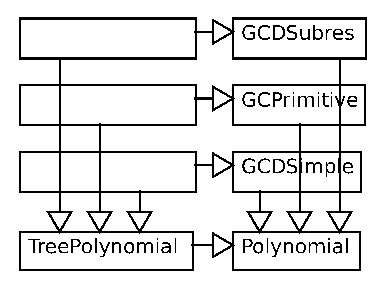
\epsfig{file=Polynomial,clip=,width=0.7\linewidth}
%\caption{Polynomial representation}
%\label{fig:poly}
%\end{figure}
%
%\subsection{Some problems solved} % -------------
%
%Mixin composition brings a solution to some code duplication related problems,
%summarized in \cite{JollyKredel:2011}, Section 3. The first one is with
%\code{SolvablePolynomial}, which should inherit nearly all its code from
%\code{Polynomial}, except just the \code{multiply()} method, rewritten in a
%non-commutative way. However, direct inheritance is forbidden by the fact that
%the class would have to inherit both from \code{RingElem\-<Polynomial<C>>} and
%\code{RingElem<SolvablePolynomial<C>>}, which is not allowed. In the new design,
%the common code is factored out in a trait which is then mixed in with both
%\code{Polynomial} and \code{SolvablePolynomial}. A similar solution is possible
%(though not yet implemented) in the case of \code{Real/AlgebraicNumber}.
%
%A second problem, also resulting in code duplication, is with multivariate
%GCD computation, see \cite{Kredel:2008}, Subsection 7.5 ``Recursive types''.
%The implementation of the algorithm as a subtrait of
%\code{MultivariatePolynomial} with a ``splitting'' capability allows to
%unify the methods \code{baseGCD()} and \code{recursive\-UnivariateGCD()}. These
%are essentially the same, except for the type of the parameters, namely:
%\code{Polynomial.Element[C]} in the base case, and
%\code{Polynomial\-.Element[Polynomial.Element[C]]} in the recursive case:
%
%\begin{verbatim}
%trait MultivariatePolynomial[C] extends Polynomial[C] {
%  def split: MultivariatePolynomial[Polynomial.Element[C]]
%}
%\end{verbatim}
%
%Here we must note that this solution would not be possible without higher-kinded
%types, another advanced feature of Scala. As we are defining several kinds of
%polynomials for each algorithm flavor or data structure representation, the
%above \code{Polynomial.Element[C]} type must be abstracted over, which mandates a
%so-called type constructor \code{T}:
%
%\begin{verbatim}
%trait MultivariatePolynomial[T[C] <: Polynomial.Element[T[C],C],C]
%    extends Polynomial[T[C], C] {
%  def split: MultivariatePolynomial[T, T[C]]
%}
%\end{verbatim}

\section{Conclusions} % --------------------------

Universal algebra can not always model all that is possible in a computer
science perspective, where program constructs which can represent and compute
with mathematical concepts, are needed. An interesting view in that respect is
the one of categories as used in Axiom, Magma and Sage. In our current,
Java-based software, a new concept for code organization in computer algebra is
proposed in the form of mixin composition, which allows to define and choose
among several algebraic computation algorithms in a modular, category-like
fashion. This category scheme ties together algebraic structures with 
some specific algorithm implementations and so solves the packaging problem.
%and data structure representations
%It also solves some long standing code duplication
%problems while still preserving type-safety.

\subsection*{Acknowledgments} %-------------------------

We thank our colleagues Thomas Becker, Wolfgang K. Seiler, Thomas
Sturm, Axel Kramer, Jaime Gutierrez, Sherm Ostrowsky, Markus Aleksy and
others for various discussions on the design of and the requirements
for JAS and ScAS. 
%Thanks also to the referees for the insightful suggestions to improve the
%paper.


\bibliographystyle{splncs}
\bibliography{com-cas}
%\balancecolumns % insert in last page

\end{document}

%%% Local Variables:
%%% mode: latex
%%% TeX-master: t
%%% End:
